\documentclass[a4paper, 12pt, twoside]{article}
\usepackage[english]{babel}
\usepackage[utf8]{inputenc}

 
%Margins
\usepackage[left=25.4mm, right = 25.4mm, top=25.4mm, bottom=25.4mm, includefoot]{geometry}
\setlength{\parindent}{0in}
\usepackage{enumitem}
\usepackage{parskip}

       
                   
%Adding Pictures
\usepackage{graphicx}
\usepackage{float}
          
                                        
%Header and Footers
\usepackage{fancyhdr}
\pagestyle{fancy}
\fancyhead{}
\fancyfoot{}
\fancyfoot[RO]{Policy Blueprint for Separation of Powers\hspace{1mm} \textbar \hspace{1mm} \thepage\ }
\fancyfoot[LE]{ \thepage \hspace{1mm} \textbar \hspace{1mm} Reforming Education Governance in India}
\renewcommand{\headrulewidth}{0pt} %change the pt width to insert header line
\renewcommand{\footrulewidth}{0pt} %change the pt width to insert footer line


%Tables
\usepackage{booktabs}
\usepackage{subfig}
\captionsetup{aboveskip=14pt,}
\captionsetup[table]{singlelinecheck = false}
\usepackage{longtable}
\usepackage{array}
\newcommand\tabitem{\makebox[1em][r]{\textbullet~}} %makes tabitem
                    
%Coloured Boxes
\usepackage{xcolor}
\usepackage{mdframed}
           
                    
%Custom Spacing
\usepackage{setspace}
         
                    
%Defining Colours
\definecolor{CCSbrown}{RGB}{163, 86, 37}
\definecolor{CCSgrey}{RGB}{105, 105, 105}
\definecolor{CCSblack}{RGB}{64, 64, 65} 
             
             
%Headings      
%Titles         
\usepackage{sectsty} %need this package for setting colours

\chapterfont{\color{blue}}  %sets colour of chapters font
\sectionfont{\color{CCSbrown}}  %sets colour of section font
\subsectionfont{\color{CCSblack}} %sets colour of subsection font
\subsubsectionfont{\color{CCSblack}} %sets colour of subsubsection font
	
    				
%Bibliography
\usepackage[authordate, backend=biber]{biblatex-chicago}
\addbibresource{new_refs.bib}
\renewbibmacro*{cite:ibid}{\printtext[bibhyperref]{\bibstring[\mkibid]{ibidem}}} 	%Getting ibid

%Hyperlinks
\usepackage{hyperref} %activates links 
\hypersetup{
colorlinks,
linkcolor = black,
citecolor = CCSbrown,
urlcolor = CCSbrown}
\usepackage{blindtext}


%Using pdf images
\usepackage{pdfpages}
\captionsetup[figure]{font=normal,skip=0pt}

%Getting landscape pages
\usepackage{lscape}		

%Preventing Hypenations
\tolerance=1
\emergencystretch=\maxdimen
\hyphenpenalty=10000
\hbadness=10000

%Fourth level of heading
\usepackage{titlesec}
\setcounter{secnumdepth}{4}
\titleformat{\paragraph}
{\normalfont\normalsize\bfseries}{\theparagraph}{1em}{}
\titlespacing*{\paragraph}
{0pt}{3.25ex plus 1ex minus .2ex}{1.5ex plus .2ex}
\setcounter{secnumdepth}{5}
\setcounter{tocdepth}{5}
\newcommand\simpleparagraph[1]{
  \stepcounter{paragraph}\paragraph*{\theparagraph\quad{}#1}}
  
  %preventing widow lines
  \clubpenalty = 10000
\widowpenalty = 10000
\displaywidowpenalty = 10000

              
              
\begin{document}
                    
%==================================================                

%--------------------------------------
%INSERTING COVERPAGE
%-----------------------------------------


\pagenumbering{gobble} %removes page numbers starting here
\pagestyle{empty} %removes footers from here onwards
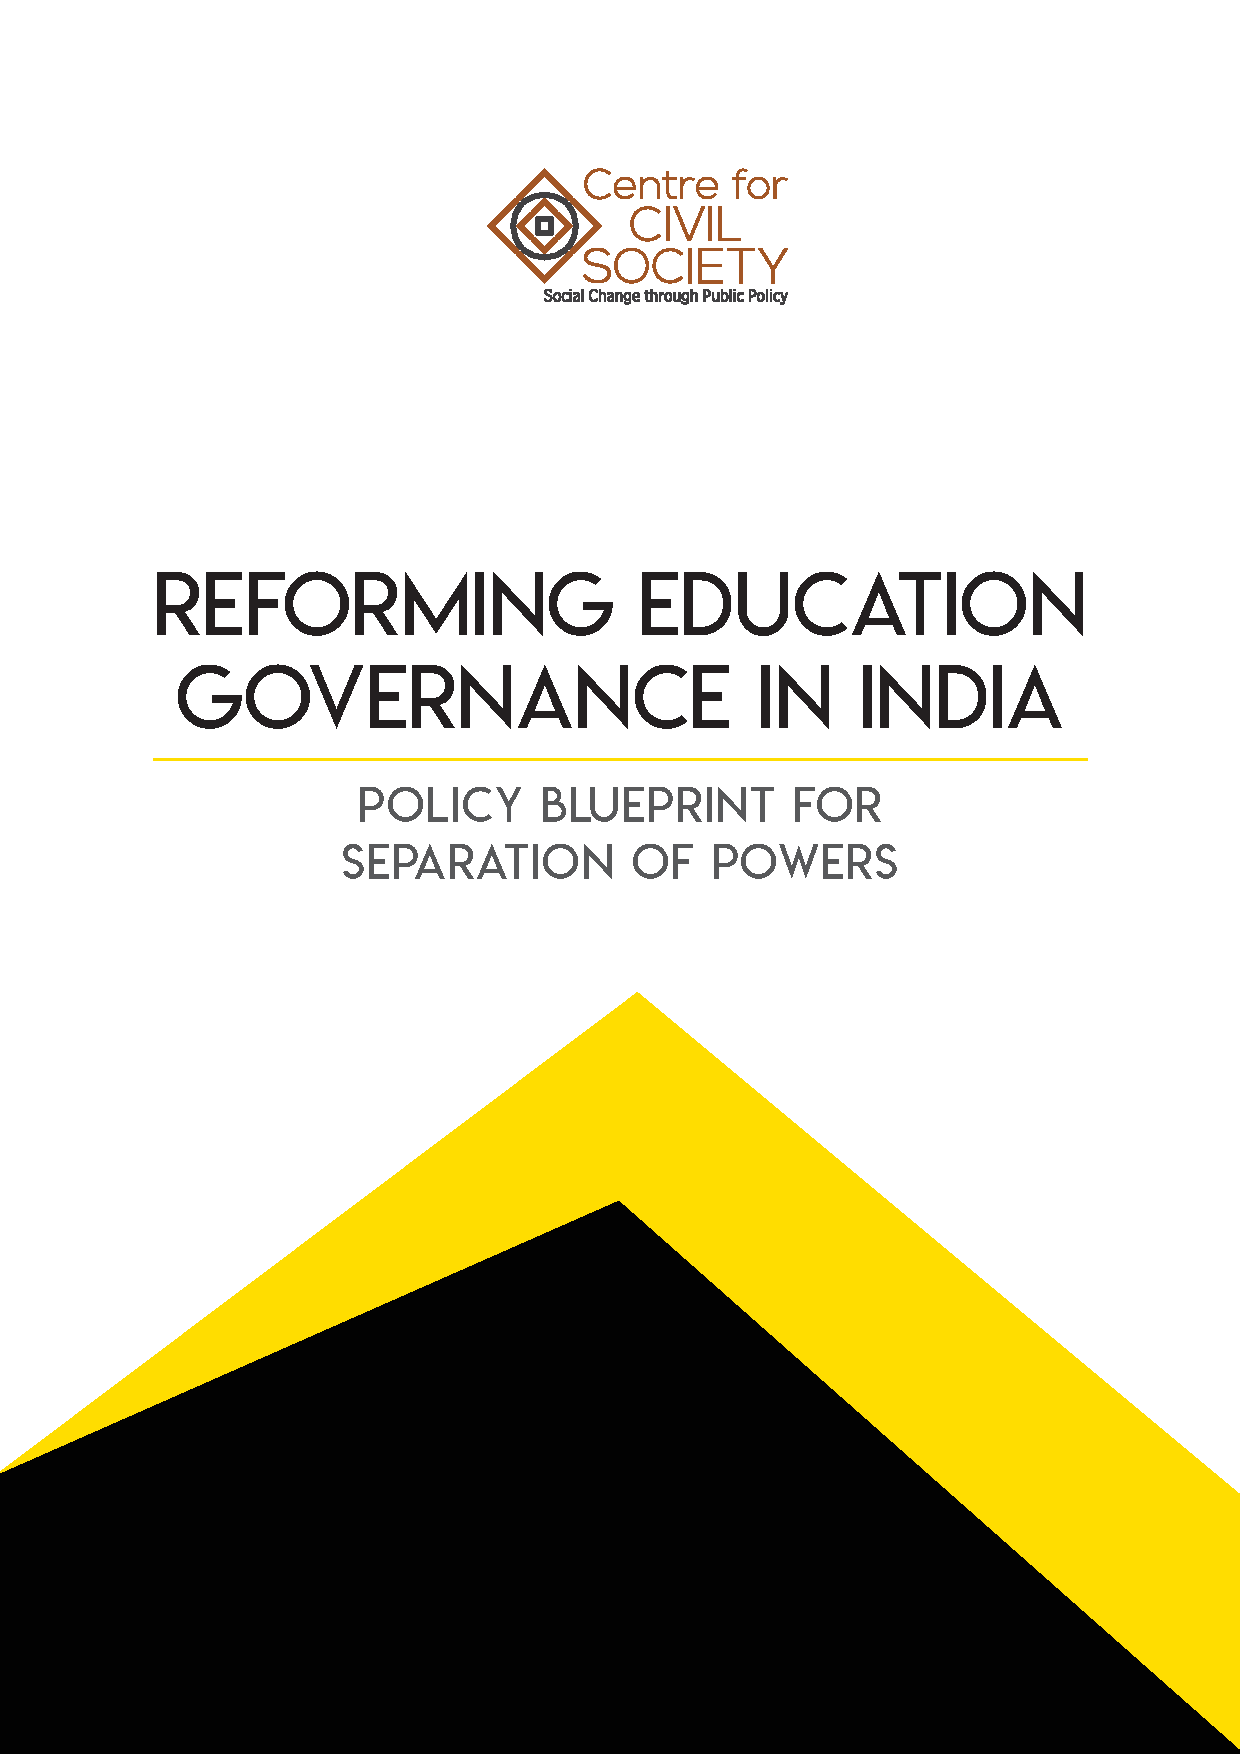
\includepdf[pages={1,2,3,4}, pagecommand={}]{Coverpage.pdf}  %attaches the pages from coverpage doc here
\pagestyle{fancy} %restarts footers from here onwards
\setcounter{page}{1} %starts counting page numbers after all the coverpages are done
\pagenumbering{arabic} %prints the new page numbers from here

  
\newpage
\newlist{abbrv}{itemize}{1}
\setlist[abbrv,1]{label=,labelwidth=1in,align=parleft,itemsep=0.1\baselineskip,leftmargin=!}

 

%=====================TOC============================                 
%This page is intentionally left blank
%\newpage    
\tableofcontents
\newpage    
\section*{List of Abbreviations}
\addcontentsline{toc}{section}{List of Abbreviations}
        
\begin{abbrv}
         
        \item[BEO]			Block Education Officer
        \item[DEO]				District Education Officer
        \item[DfE]			Department for Education
        \item[DoE]				Director of Education
        \item[DoT]			Department of Telecommunications
        \item[GCERT]				Gujarat Council of Education Research and Training 
        \item[MLA]				Member of the Legislative Assembly
        \item[MoE]				Ministry of Education 
        \item[NTP]				National Telecom Policy
        \item[OECD]			Organization for Economic Cooperation and Development
        \item[OFQUAL]			Office of Qualifications and Examinations Regulation
        \item[OFSTED]			Office for Standards in Education
                \item[PISA]			Program for International Student Assessment
        \item[RTE]				Right of Children to Free and Compulsory Education Act 2009 
        \item[SAT]				Securities Appellate Tribunal
        \item[SCERT]			State Council for Education Research and Training
        \item[SEBI]				Securities and Exchange Board of India
        \item[SIS]				State Implementation Society
        \item[TDSAT]			Telecom Dispute Settlement and Appellate Tribunal
        \item[TRAI]			Telecom Regulatory Authority of India
        \item[UK]		United Kingdom
              
        
         
\end{abbrv}
\newpage        

                    
%======================LIST OF ABBREVIATIONS==========     
%Executive Summary
\newpage
\section*{Executive Summary}
\addcontentsline{toc}{section}{Executive Summary}
                    
                  From 2010 to 2014 the per-student expenditure increased by 10\% CAGR (\cite{aibb2013-14}; \cite{cprbb2017-18}). Yet, enrolment in government schools decreased by 11.1 million, and in private schools, rose by 16 million. Parents are choosing fee charging private schools over free government schools despite both having poor learning outcomes. The cost to outcome ratio in government schools points to a governance problem: of poor value for money in government expenditure on education.

Fixing this requires an urgent restructuring of the governance of education. Three ideas need to be considered—direct education funding to every student, separation of powers in education administration, and learning outcomes based recognition of schools. In this brief we discuss one of these three ideas: separation of powers.

Even NITI Aayog aims to “lay down the foundation for a long-term strategic change” in the next three years, and recommends “separation of functions” as a key reform idea \parencite{niti3yearagenda}.\footnote{ In the political realm the term is Separation of Powers, in administration, Separation of Functions or Roles, and in business, Segregation of Duties. In this paper, the phrases are used interchangeably, but invoke the original idea: incompatible powers/functions/roles should be separated into distinct entities.}

Separation of powers is one of the foremost principles of good governance. The idea behind separation of powers is that the rule-maker, rule-executor and adjudicator should be distinct from each other. Such a separation installs checks against conflicts of interest by regulatory authorities, improves service delivery, and increases institutional accountability for outcomes. 

The principle has been repeatedly upheld by the Indian courts as a cornerstone of the rule of law. In sector after sector, the doctrine has been applied systematically to improve the effectiveness and efficiency of public service delivery.

The implementation of the principle of separation of powers in institutions is called \textit{uncoupling} and comes about through thoughtful agency redesign.

When implemented in a government administrative department, \textit{steering} functions (that \textit{set} the course of action), such as formulation of policy and regulation, are separated from \textit{rowing} functions (that \textit{execute} the course of action), such as service delivery and enforcement of rules.\footnote{‘Service delivery’ functions relate to the daily operational tasks in the running of government schools. ‘Compliance’ functions relate to the monitoring of the performance of ‘service delivery’ functions.} 

We need to \textit{uncouple} the functions exercised in the governance of the school education sector of India, particularly at the state level. A state government’s Education Department is responsible for the construction of schools, teacher hiring and management, distribution of funds for school activities and formulation of state-level education policy.
\\

Separation of powers in education will address three persistent problems.

\textbf{First, it will increase compliance with policy, laws and rules by increasing a school inspector’s focus on enforcement.} Currently, a school inspector’s primary responsibility, i.e. ensuring compliance with education standards, is interrupted by “collecting donation, in cash or kind, for the benefit of education”, “handling pension cases”, “opening GPF accounts of newly appointed teachers” and “maintaining service books of teacher” \parencite{deo_chart}. Of the inspector’s work-time, only 40\% is spent on supervision and inspection; of which, only 8.7\% is on supervising teachers. Increasing time on inspection can also lead to substantial gains in efficiency of public spending and better outcomes. Conducting inspections even once in three months can reduce teacher absenteeism by about 27-35\%, could save India could save \$1.5 billion annually \parencite{karthik_m_10b}. 

\textbf{Second, it will facilitate school choice for low-income parents.} Currently, state government Education Departments are suspicious about low-fee private schools and regularly issue closure notices \parencite{nisa}. When the department is the appellate authority against its own orders, private schools are likely denied a fair hearing against forced closure. Moreover, a policy maker’s implicit bias against private schools may affect impartial oversight and governance of all schools.

\textbf{Third, it will hold all schools accountable for their learning outcomes.} When an independent agency assesses the learning outcomes of all schools and publishes results in the public domain, the funding of these schools can be linked to outcomes. In the private school market, assessment information can empower parents to hold schools accountable.

Three reforms are required to effect the separation of powers in education:

\begin{enumerate}[noitemsep]

\item Transferring the running of government schools to an independent public organisation;

\item Setting up an adjudication tribunal to settle challenges to rules and enforcement; and

\item Granting autonomy to the State Council for Education Research and Training (SCERT) for assessment of learning outcomes.

\end{enumerate} 

Such separation has been systematically instituted in telecommunications where BSNL and MTNL, government-owned service provider are independent from the Ministry of Communications, and the Telecom Regulatory Authority of India (TRAI) regulates both public and private sector companies equally. It was also applied to the financial sector in India, and in the case of education governance in the UK, Denmark, Sweden, Chile, Mexico, Australia and Emirate of Dubai. In England and Chile, the Office for Standards in Education (OFSTED) and the Superintendent of Education, respectively, enforce the law for both public and private schools. 

In this brief, we discuss ideas on separation of powers in a typical state government Education Department and separation of roles of sub-state level functionaries. The Blueprint is organised into six sections: one outlines the governance of education in India; two describes the problem and the manifest consequences; three outlines a solution to the problem; and four gives examples of similar solutions in other countries.

          

%Introduction
\newpage
\section*{Introduction: Governance of India's School Education}
\addcontentsline{toc}{section}{Introduction: Governance of India's School Education} 
                    
The education system of India has consistently delivered poor learning outcomes. When the Program for International Student Assessment (PISA) evaluated India in 2009, it ranked our students at 73\textsuperscript{rd} out of 74 countries (just above Kyrgyzstan) \parencite{pisa2009}. 

This clarion call for switching the focus of education policy from inputs to outcomes went unheeded. India continued on the same path and passed the input centric Right to Free and Compulsory Education Act of 2009 (“RTE”) in 2010. The per-student expenditure in government schools consistently rose at 10\% CAGR from Rs. 2,455 in 2010 to Rs. 4,385 in 2016 \parencite{ai1819}. In the same period, the percentage of class 8 students who could read a class 2 text in these schools fell from 82\% to 70\% (\cite{aser2016}). 

The largest share of the additional expenditure on education from 2010-2016 was on government teacher salaries followed by infrastructure (\cite{aibb2013-14}; \cite{cprbb2017-18}). This is strong evidence that continuing on the same track is not a solution; neither is spending thoughtlessly on technology. There is a need to restructure governance of the education system. 

In sector after sector across the world, new public management principles have been applied to increase transparency, accountability, efficiency and effectiveness of government services. One of the core ideas in new public management is \textit{uncoupling} or the separation conflicting government functions and assigning them to distinct and/or independent agencies. The separation not only facilitates better execution but also creates an internal system of checks and balances. The idea is applied extensively in the administration systems of UK, New Zealand and Canada \parencite{uncoupling}, and education governance of Denmark \parencite{denmarkgovernance}, Sweden \parencite{sweden_governance}. 

\textit{Uncoupling} is the application of the doctrine of \textit{separation of powers} to administration of government departments. In this paper, we describe the structure of education governance in India, its different functions and their incompatibility, consequences of the incompatibility, and ideas for applying \textit{uncoupling} to solve the problem. 
                    
                    
\newpage 
%Roles of Central, State and Local Governments in Education
\subsection*{\raggedright Roles of Central, State and Local Governments in Education}   
\addcontentsline{toc}{subsection}{Roles of Central, State and Local Governments in Education}                
                    
Education (including school, university, technical, medical and vocational) falls under the concurrent list in India; both the central and state governments can legislate on the subject.\footnote{Refer: The Constitution (Forty-second amendment) Act, 1976.} The central government sets the general direction of education policy and lays down governing tenets and principles, and the state governments frame their respective legislation within the framework of the central government’s policy. The responsibility for policy execution rests chiefly with state governments.
%Figure 1
\begin{figure}[H]
 \centering
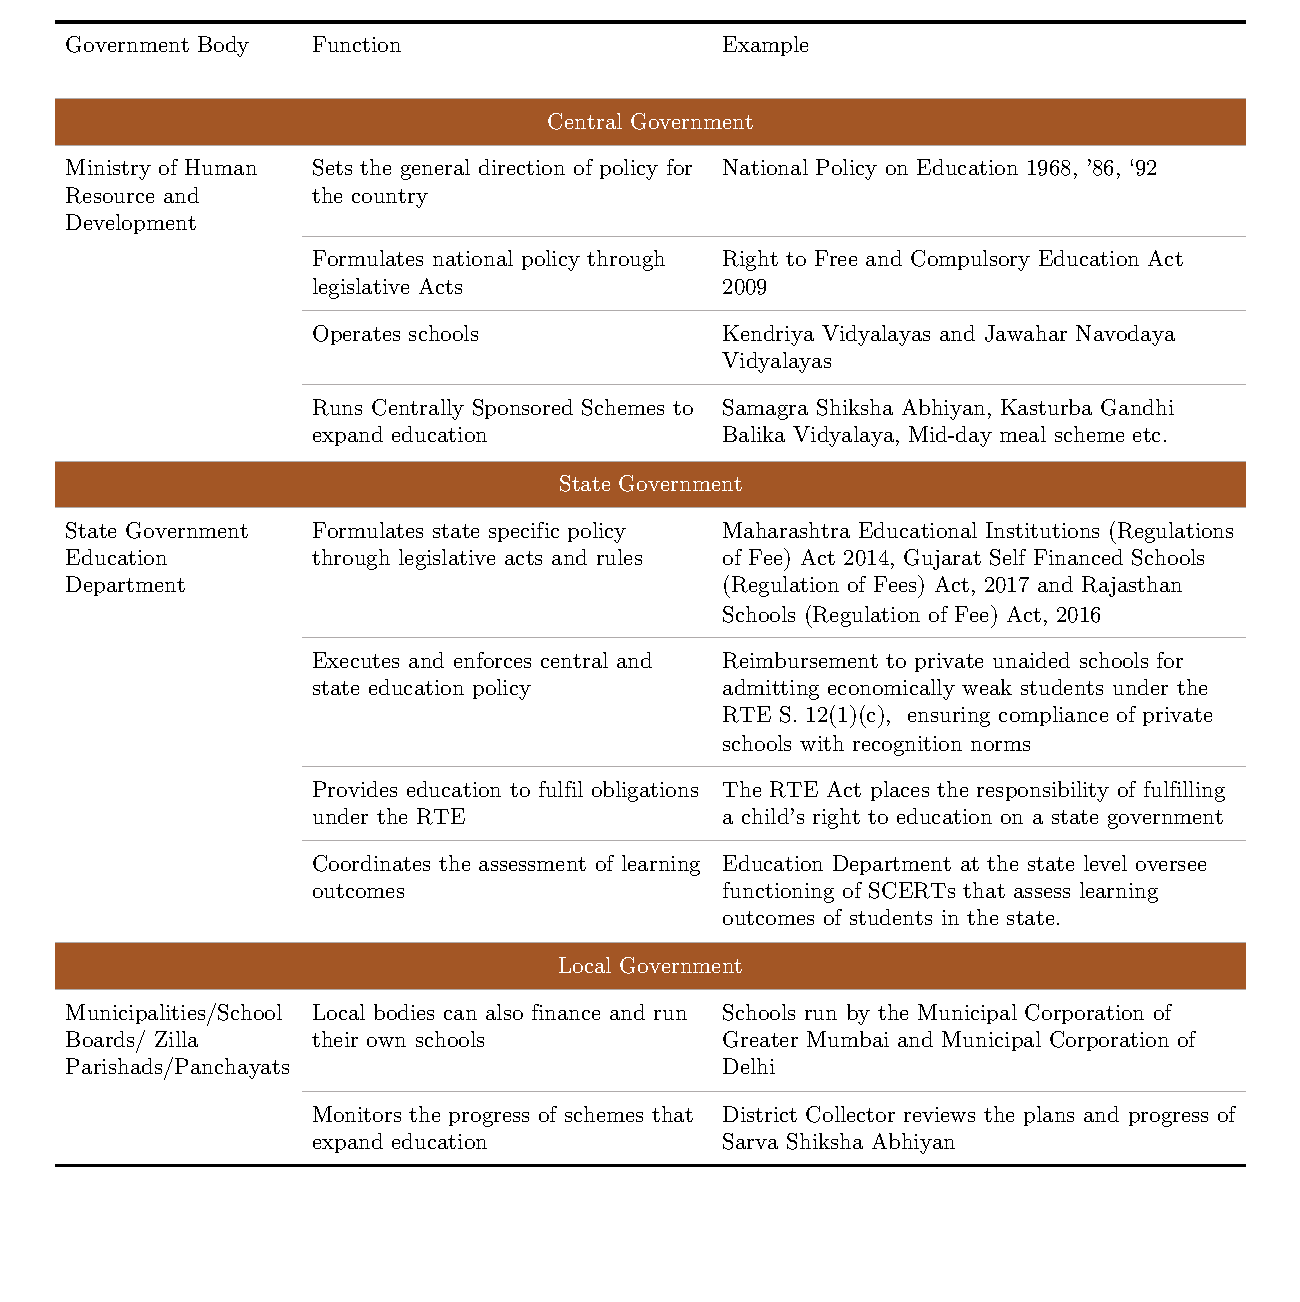
\includegraphics[page=1, height = 16cm]{figure1}
\caption{Education related functions of the three levels of government}
\end{figure}
                    
                    
%Functions of the State Government Education Department
\subsection*{\raggedright Functions of the State Government Education Department}  
\addcontentsline{toc}{subsection}{Functions of the State Government Education Department}  

A state government’s Education Department\footnote{While department titles may vary across states,throughout this paper, we use this title to describe the education department in any state.} heads the administrative setup that executes the policy mandate for school education. A typical state government Education Department is usually set up into sub-departments called Directorates based on the level of education.\footnote{Across India, school education is typically divided into three levels–elementary (classes 1 to 8) secondary (9 and 10) and higher-secondary (11 and 12)– and based on the state’s preference, single or multiple sub-departments oversee each level.} The Directorates are headed by a Director who reports to the Principal Secretary of Education.

%Figure 2
\begin{figure}[H]
 \centering
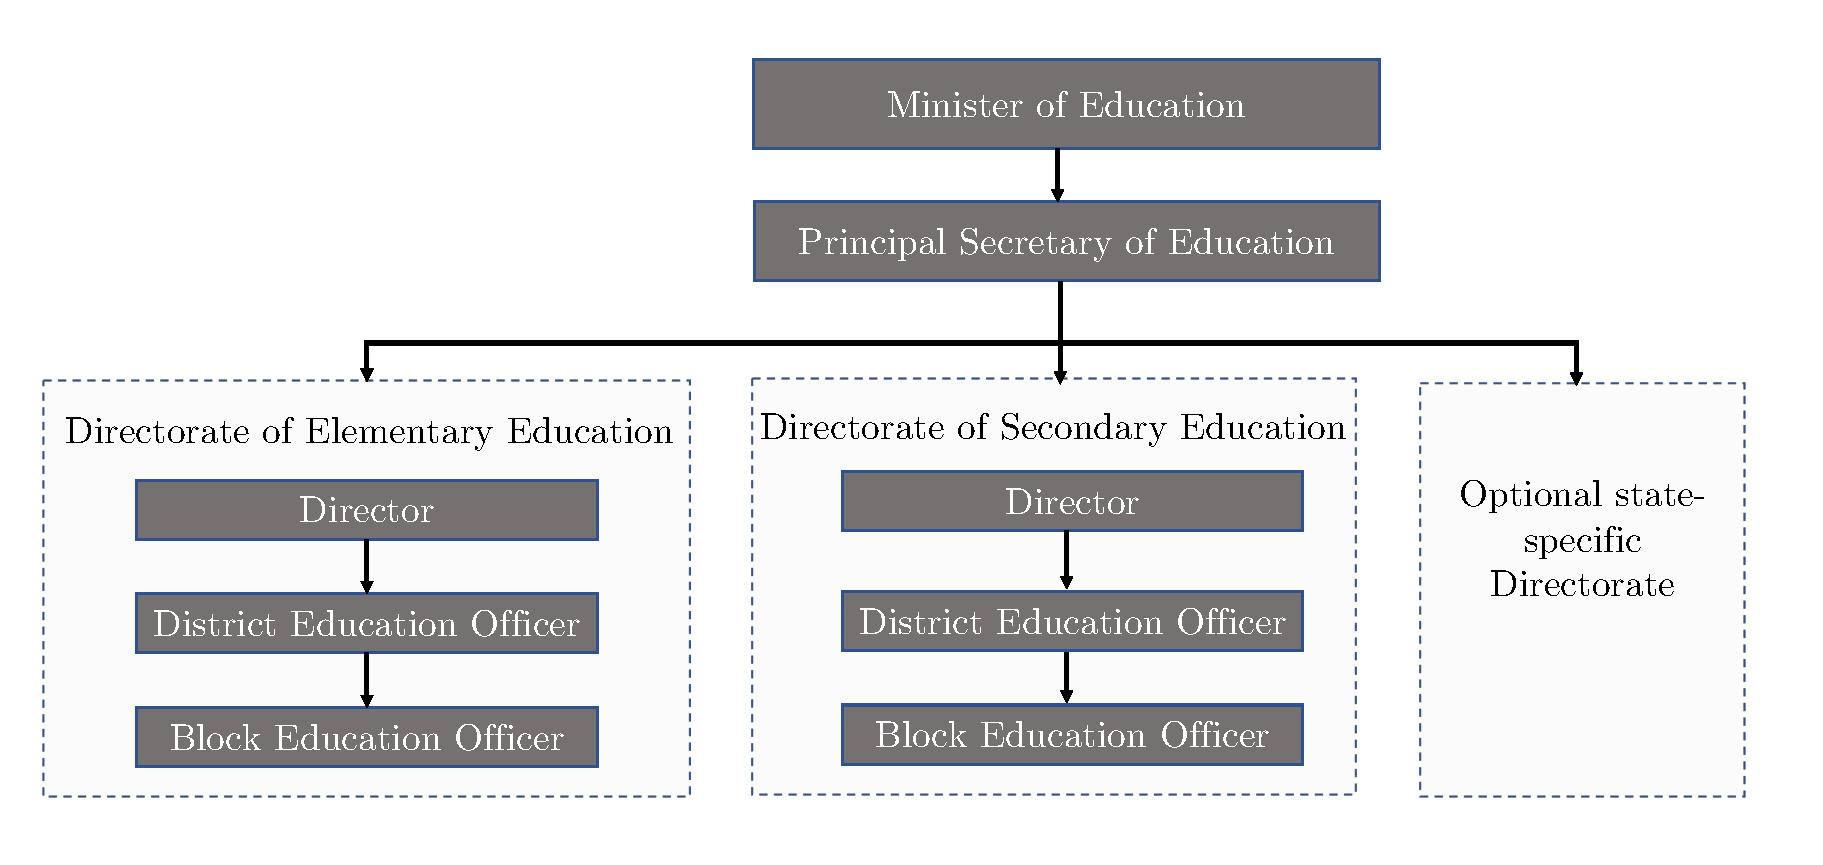
\includegraphics[page=1, width = 16.5cm]{figure2}
\caption{Functionaries in a typical state government Education Department}
\end{figure}

In the process of executing the policy mandate, functionaries of a state government Education Department perform six diverse functions.

\begin{enumerate} 
\item \textbf{Policy-formulation:} This comprises the framing of Legislative Acts (statutes) and drafting of corresponding executive orders that apply only within the state. 

\begin{enumerate}
%Framing legislative Acts
\item \textbf{Framing Legislative Acts:} Elected representatives in the state assembly (MLAs) pass state laws set within the broad framework of the central government’s policy. The Maharashtra Employees of Private Schools (Conditions of Service) Regulation Act, 1977 to regulate the salaries and employment of private school teachers and the Andhra Pradesh School Education (Community Participation) Act, 1998 to ensure community participation and achieve the goal of universal primary education are examples of state level Legislative Acts. 

\newpage
%Drafting subordinate legislation
\item \textbf{Drafting Subordinate Legislation:} Subordinate legislation outlines implementation details attached to the Act. It can only be framed under a central or state Act if the Act gives rule-making power to the government \parencite{exec_rule_making}. The Principal Secretary of Education at the state government drafts and passes rules, regulations, bye-laws, orders, and notifications in consonance with central and state government Acts. 

For example, after the  Haryana School Act 1995 was passed, the Department of Education passed the Haryana School Education Rules, 2003. Similarly, the central government passed the RTE Act in 2009 and drafted ‘model rules’ for the states to refer. While many states adopted the model rules as is, some states added additional provisions.\footnote{For a comprehensive comparison, please refer to Centre for Civil Society’s RTE Rule Matrix: \href{https://bit.ly/2qRvlJ7}{https://bit.ly/2qRvlJ7}} For example,  Uttar Pradesh, notified about 40 different conditions a private school to fulfil in order to gain recognition under its RTE rules (Link to order: \href{https://bit.ly/2DMyu5g}{https://bit.ly/2DMyu5g}).

\end{enumerate}
%service delivery
\item \textbf{Service delivery:} The function is carried out by the Directorates of Education and entails the organisation and management of state government-owned schools including construction and upkeep of school infrastructure, providing free books, meals and scholarships, hiring teachers and teaching students.\footnote{There are other publicly funded schools India run by the central government (Kendriya Vidyalayas, Jawahar Navodaya Vidyalayas, Army Public Schools), local governments (Zilla Parishad (district level local authority) and authorised municipalities) and the state tribal welfare departments. But the service delivery in these schools is not the responsibility of the state government Education Department.} The Directorates are staffed by the Director of Education (DoE),\footnote{A state can have one or multiple Directorates based on the governance structure, and their title may vary with states.}  District Education Officers (DEOs) and Block Education Officers (BEOs), and report to the Principal Secretary of Education.

The state government Education Department executes its service delivery function through the State Implementation Society (SIS) of the Samagra Shiksha Abhiyan scheme.\footnote{Samagra Shiksha Abhiyan was formed by merging the erstwhile Sarva Shiksha Abhiyan, Rashtriya Madhyamik Shiksha Abhiyan and Scheme of Restructuring and Reorganisation of Teacher Education.} Although SIS is an autonomous Society at the state level, it is under the administrative control of Directorate of Education, and led by DEOs and BEOs at the district and block levels \parencite{ssa_guide}. In states like Jammu and Kashmir, it is given the status of a Directorate \parencite{jnk_ssa}.  
%financing
\item \textbf{Financing:} This includes the allocation and disbursement of public funds to execute the state government’s service delivery function. Central and state governments together finance two cost centres under service delivery: state government Education Department and SIS.

\textbf{Financing the state government Education Department:} Funds from the Centre are transferred to the state government’s treasury and are supplemented by the state government’s education budget. These funds pay for staff salaries, administrative office expenses, salaries of government school teachers, reimbursement to private unaided schools for admitting economically weaker students under the RTE Act and other state-specific welfare programs or needs.

\textbf{Financing the State Implementation Society:} The central government directly funds the SIS. Subsequently, a matching amount is deposited by the state government’s Department of Finance. SIS then transfers these funds to the district level for expenses on construction and maintenance of classrooms and infrastructure, provision of free books and other child welfare services \parencite{ssa_css}. 
%compliance
\item \textbf{Compliance:} Relates to the enforcement of education policy in the state, and includes suo-motu inspections to monitor compliance with rules, investigation of complaints and prosecution of the policy violators. This function is carried out by DoE, DEOs and BEOs under the supervision of the  Principal Secretary of Education. The enforcement power of these officials is not only against violators in the public education services but also against all private schools in the state.
%adjudication
\item \textbf{Adjudication/Dispute resolution:} This refers to judicial action of upholding or overturning any order or penalty (monetary and non-monetary) imposed by the state government against the stakeholders in education (teachers, parents, students and private school owners). For orders passed under certain Acts/rules, the executive branch of the state government itself is the appellate authority and its decision on the matter is final.
%assessment
\item \textbf{Assessment:} This includes the monitoring of learning outcomes to determine the competency of students. The SCERT is responsible for administering an annual assessment to a sample of students to determine their learning outcomes.\footnote{The National Council for Educational Research and Training administers the National Achievement Survey to assess the learning outcomes. However, at the state level, the SCERTs are responsible for administering the survey to a sample student population.} 

\end{enumerate}

%Where does the problem lie?
\section*{Where does the problem lie?} 
\addcontentsline{toc}{section}{Where does the problem lie?}     
\subsection*{Simultaneous execution of multiple incompatible functions}
\addcontentsline{toc}{subsection}{Simultaneous execution of multiple incompatible functions}       

These six functions of the state level Education Departments in India are fundamentally incompatible, create conflict of interests and reduce the overall efficiency of the system. However, one department performs all six using functionaries from within the department, and often assigning individual functionaries many of these six incompatible functions. 

Incompatibilities and conflicts arise in the following ways:

\begin{enumerate}

\item The service deliverer (one who runs government schools) should be held accountable by the financier (one who allocates the public funds) for the usage of public funds, and by the enforcer (one who enforces rule compliance on teacher attendance, classroom size, learning outcomes etc). But where each of these roles is collapsed into one department or functionary, accountability is lost.

\item The validity and legality of rules and any abuse of power during compliance is to be checked by the adjudicator. But when the one who makes the rules or passes the compliance order also adjudicates on it, the channel for seeking relief becomes ineffective and cannot be relied on for objectivity and impartiality. 

\item The purpose of assessment is to test the quality of performance by the service deliverer. But when the service deliverer tests himself, the credibility of the assessment is questionable.

\end{enumerate}          
 
%Results of this execution model                               
\subsection*{Results of this execution model} 
\addcontentsline{toc}{subsection}{Results of this execution model}       

When a single department performs six incompatible functions, it diminishes accountability and eliminates checks and balances on the discharge of different responsibilities. When a single functionary in the department performs more than one function in the absence of independent checks, it leads to conflicts of interest and reduces efficiency of performance. 

\subsubsection*{1. Violation of natural justice}
\addcontentsline{toc}{subsubsection}{1. Violation of natural justice}   

When the entity in-charge of enforcing compliance hears appeals against its own enforcement actions, the process goes against the first principle of a fair hearing and trial: the right to independent, impartial and competent judges. The principle is grounded in the natural justice argument that \textit{no one shall be a judge in his own cause.}

This principle is violated in the case of avenues to appeal against a state government Education Department’s refusal to grant school recognition certificates or their threats to withdraw recognition.\footnote{Recognition certificates are granted by the state education department to private schools. The RTE Act made it mandatory for all private schools to have the recognition certificates in order to function. See  Section 18(1) of the RTE Act. } For example, the Haryana School Education Rules 2003, assign power to the Director of Education to  withdraw recognition certificates of a private school,\footnote{See Rule 43(1) of Haryana School Education Rules, 2003.} and the power to hear appeals against withdrawal proceedings or closure notices to the Principal Secretary.\footnote{See Rule 43(4) of Haryana School Education Rules, 2003.} 

It is often difficult to prove the actual bias in a decision of the Principal Secretary. For example, in A. V. Public School and Ors. vs. State of Haryana (2015), the High Court of Punjab and Haryana intervened against unreasoned orders issued by the Haryana Education Department. The mass closure notices issued by the department were overturned as they did not follow due process of stating the violations on the notices and considering replies of the schools to the show cause notices. The court held “whatever were the failings of the petitioners, there is a modicum of procedure that the State is bound to follow before the orders are passed directing closure of the schools. If only the State had undertaken any inspection and noticed on a case to case basis that norms had not been fulfilled or applications had not even been filed or replies had not been given, it would not be possible for the State to pass the order in the manner that it did.”

The courts in India have upheld even a reasonable suspicion of bias as undesirable. In Shyam Singh vs. The State of Rajasthan and Anr. (1972), the High Court of Rajasthan held, “the question is not whether a bias has actually affected the judgment. The real test is whether there exists a circumstance according to which a litigant could reasonably apprehend that a bias attributable to a judicial officer must have operated against him in the final decision of the case.”

%3. Ineffective performance monitoring and rule compliance
\subsubsection*{2. Ineffective performance monitoring and rule compliance}
\addcontentsline{toc}{subsubsection}{2. Ineffective performance monitoring and rule compliance}

Teacher absenteeism in government schools of India was recorded at 25\% \parencite{kremer_absence}, and the cost to the taxpayer was estimated at \$1.5 billion annually \parencite{karthik_m_10b}. Research estimates that a 5\% increase in the absenteeism rate of teachers who stayed with the same class for two years reduced student gains by 4-8\% during the year \parencite{das2007teacher}. 

State government school education inspectors\footnote{The district and block level education officers (DEOs and BEOs) are the education inspectors.} have been unable to check the levels of teacher absenteeism in the classroom despite evidence that of all the variables that affect student performance, teacher presence in the classroom has the highest correlation with performance \parencite{wilmawadhwa}.

OECD’s Inspection Toolkit specifies that a good inspection system ought to have clear non-conflicting roles, skilled and trained inspectorate force, random allocation system, accountability for performance and a system to ensure compliance \parencite{toolkit}. However, the inspection system of the state government Education Department fails at the first step: clarity of job descriptions (\cite{deo_chart}, Appendix 2).
 
School inspectors currently perform numerous activities unrelated to inspection such as “collecting donation, in cash or kind, for the benefit of education”, “handling pension cases”, “solving cases related to unaccounted for and extra leave taken by the teachers” and “maintaining service books of teacher”. While some of these tasks pertain to compliance, most relate to service delivery. The job chart for a School Inspector lists 36 such distinct tasks that do not clearly focus on inspections. 

The time on task of frontline education officers shows the tradeoff between inspection and non-inspection related tasks. The data is reproduced in Figure 3 (\cite{timestudy_beo}).


%Figure 2
\begin{figure}[H]
 \centering
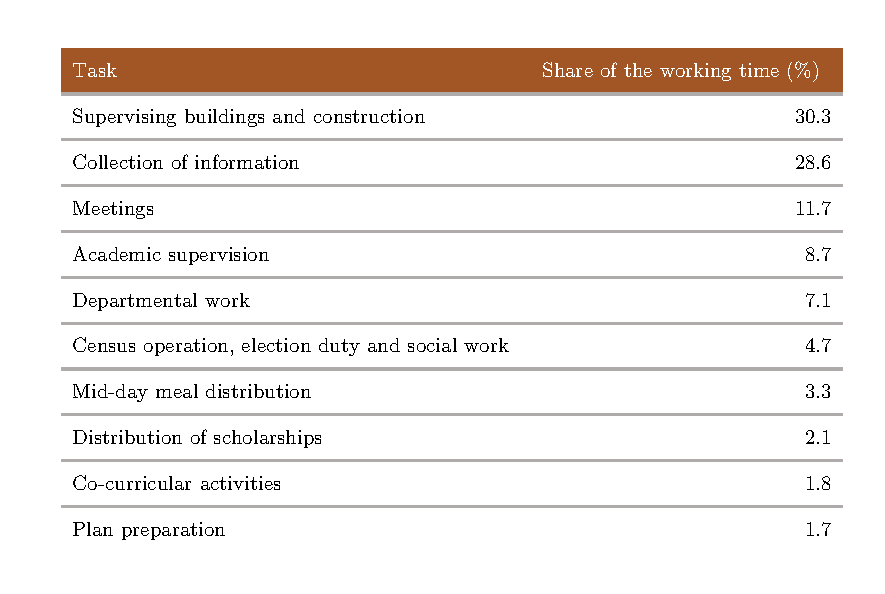
\includegraphics[page=1, width = 16cm]{figure3}
\caption{Average share of time on tasks of 133 Assistant Basic Education Officers from Uttar Pradesh}
\end{figure}

30.3\% of an inspector’s time is estimated to be spent on supervising construction of buildings and only 8.7\% on academic supervision. Supervision of building construction requires domain expertise and effort to hold building contractors accountable for public funds. Similarly for  academic supervision. The steps to provide training and imbibe skills, and establish accountability mechanisms become futile if the same person is responsible for different niche supervisory roles, but also spends most of their time on non-supervisory functions.

\subsubsection*{3. Differential laws for government and private schools}
\addcontentsline{toc}{subsubsection}{3. Differential laws for government and private schools}  

The RTE Act and its attached rules have set discriminatory standards for private and government schools. In addition, the state government Education Department both runs government schools and enforces these discriminatory standards.

While the RTE Act requires all schools to comply with the prescribed norms on pupil-teacher ratios, infrastructure and teacher-qualifications, the consequences of violating the norms are different for government and non-government (private) schools. Section 18 of the RTE Act stipulates that no private unaided school can be established or continue to function without obtaining a certificate of ‘recognition’ from the state government Education Department, and Section 19 lays down the various penalties (including closure) for non-compliance with the given conditions. While Section 8(g) of the Act specifies as the state’s duty to ensure that government schools also conform to the norms of the Act, there are no penalties if they do not. Thus, there is no incentive for the government schools to comply with the norms. In response to a 2016 parliamentary question, the Ministry for Human Resource Development stated that only 6.4\% of government schools in the country fulfil the recognition norms \parencite{64_RTE}. 


%How do we fix the problem?
\section*{How do we fix the problem?}
\addcontentsline{toc}{section}{How do we fix the problem?}
\subsection*{Applying the approach of \textit{Uncoupling}}
\addcontentsline{toc}{subsection}{Applying the approach of \textit{Uncoupling}} 

Education in India today faces several problems such as poor learning outcomes, high teacher absenteeism, lack of parental choice and low efficiency of public expenditure. Given this, small incremental changes in input-norms, spending on infrastructure and introducing gadgets for governance are neither fit for purpose nor feasible. A fundamental rethinking of governance is required. 

NITI Aayog concurs that the need of the hour is “governance that enables the system to operate smoothly” and recommends ‘separation of functions’ \parencite{niti3yearagenda}. We recommend a three-step \textit{uncoupling} approach to implement NITI’s topline recommendation:


\begin{enumerate}
\item Classify the state government Education Department’s functions as steering or rowing functions; 

\item Retain regulatory and compliance enforcement functions within the department, and prepare for independent discharge mechanisms for other functions; and

\item Design independent agencies thoughtfully to discharge service delivery, adjudication and grievance redressal, and assessment.
\end{enumerate}

David Osborne and Peter Plastrik argue that “\textit{Uncoupling} separates policy making and regulatory roles (steering) from service delivery and compliance roles (rowing), while also separating service delivery functions from compliance functions. This helps steering organizations concentrate on setting direction and frees rowing organizations to concentrate on achieving one or two clear missions” \parencite{uncoupling}. 

\newpage
%Three step process to effect separation
\subsection*{Three step process to effect separation}
\addcontentsline{toc}{subsection}{Three step process to effect separation} 
\subsubsection*{1. Classify department functions as \textit{steering} or \textit{rowing}} 
\addcontentsline{toc}{subsubsection}{1. Classify department functions as \textit{steering} or \textit{rowing}}    

Within government administration, functions that set policy objectives and draft the rules of the game are steering functions, and those that execute the policy direction, are rowing functions.

\textit{Steering} functions include the formulation of systemic objectives and law, and the drafting of subordinate legislation and regulation (including government orders, rules under statutes, guidelines etc) by the executive. 

Within the executive branch, \textit{rowing} functions relate to the implementation of the objectives and policy mandate set by the steering functionaries. Among others, these functions include, service delivery responsibilities such as the management of government owned and operated services,\footnote{‘Service delivery’ functions relate to the daily operational tasks, in order to perform the welfare activities of the Ministry.} and monitoring compliance and enforcing rules.\footnote{‘Compliance’ functions relate to the monitoring of the performance of ‘service delivery’ functions.} 

Using this conceptual framework, we classify the functions of three main functionaries in a state government Education Department in Figure 4.

%Figure 4
\begin{figure}[H]
 \centering
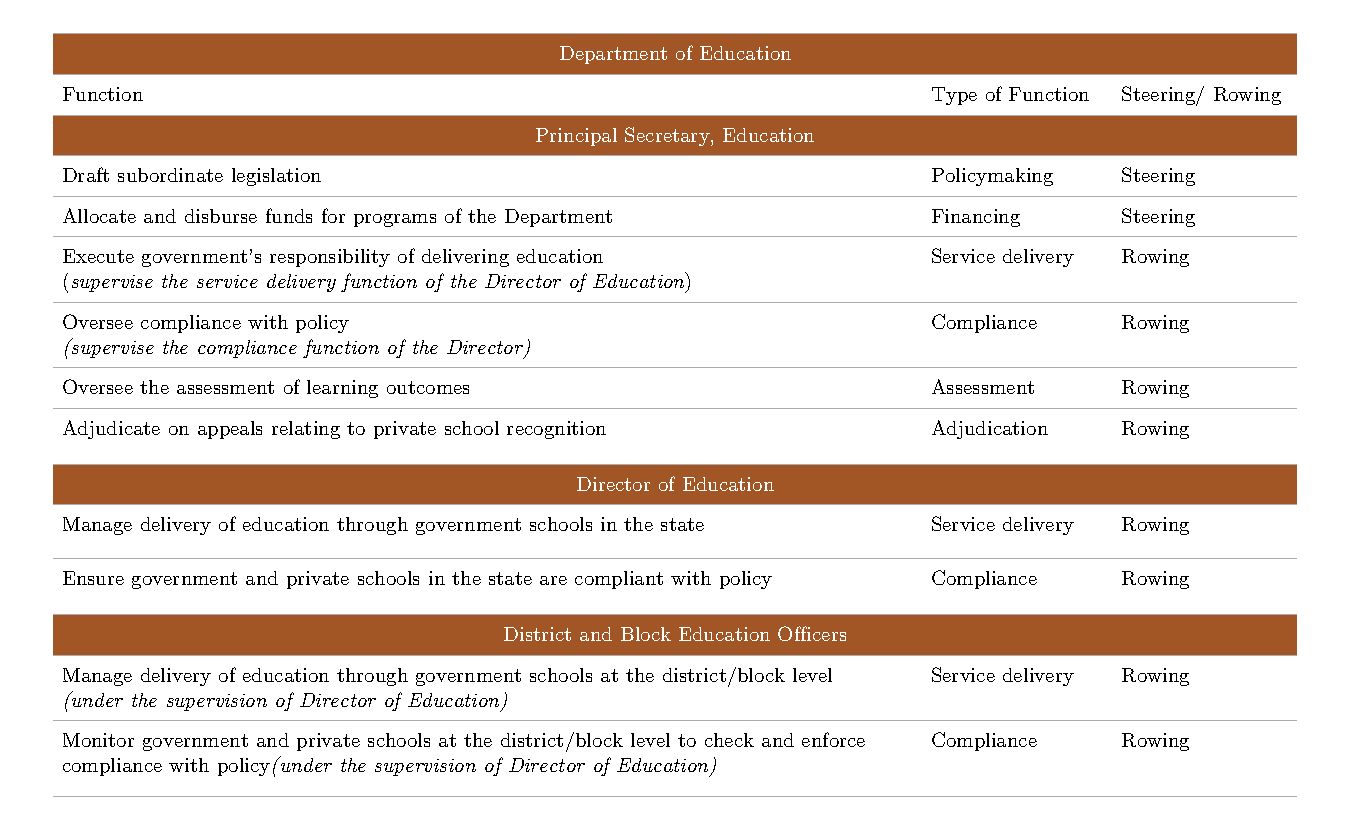
\includegraphics[page=1, width = 16.2cm]{figure4}
\caption{Classification of the state government Education Department’s functions into steering and rowing}
\end{figure}



%Regulatory and compliance functions stay in situ, others get redesigned
\subsubsection*{2. Regulatory and compliance functions stay in situ, others get redesigned} 
\addcontentsline{toc}{subsubsection}{2. Regulatory and compliance functions stay in situ, others get redesigned}     

Once functions are labelled clearly, it is easy to see points of conflict and tension. The separation of powers and functions preserves the rule of law, prevents conflicting interests from acting and the resulting clarity of roles ensures accountability in the system. \textit{Uncoupling} steering and different rowing functions helps eliminates the tension between roles that compromises the overall quality of the institution. 

\textit{Uncoupling} then asks which functions ought to be retained for discharge inside the state government Education Department and which ones ought to be separated out to independent agencies. 



\textbf{Retain regulatory, financing and compliance functions:} The state government Education Department works alongside the legislature to draft the overall vision and objectives of policy. As the executive, it also bears overall responsibility for ensuring the objectives are met. Therefore, the function of drafting subordinate legislation and ensuring \textit{compliance} (using the state’s power to pass and enforce orders) could be retained within the department.



In Figure 5, the Principal Secretary of Education is responsible for the \textit{steering} functions and also the \textit{rowing} function of overseeing compliance with policy. However, power to monitor and enforce compliance is delegated to the Director of Education.\footnote{See: Delegation of Powers under the Delhi Act and Rules, 1973 (Link: \href{https://bit.ly/2Bg5h0d}{https://bit.ly/2Bg5h0d})} 

\begin{enumerate}
\item \textbf{Separate the service delivery function:} As the department will enforce compliance, it should not perform the service delivery function. The service delivery function of building and running schools, teaching students and providing other welfare measures ought to be separated out into a distinct agency. NITI Aayog recommends the formation of a separate publicly owned agency for service delivery (\cite{niti3yearagenda}, p. 137).

\item \textbf{Separate the assessment function:} State government Education Departments periodically carry out learning assessments of sample student populations to gauge learning and competency levels of students. Assessments need to be conducted by an independent and impartial agency to objectively evaluate the students, and point out the success in achieving systemic goals and effectiveness of public spending. At the state level, the SCERTs administers the National Achievement Survey to assess the learning outcomes. SCERTs, however, despite being conceptualised and established as independent institutes, are under the administrative control of either the Principal Secretary of Education or Directorates of Education \parencite{scerts}. For example, the SCERT in Karnataka is given the status of a Directorate in under the Principal Secretary and is overloaded with administrative work \parencite{scert_structures}.

\item \textbf{Separate the adjudication function:} Currently, the power to adjudicate on withdrawal of (or refusal to grant) recognition certificates to private unaided schools rests with the executive branch. Adjudication of any order issued by the state government’s Education Department should be done outside of the department’s control, where the Department is treated as an equal party to a dispute. 

\end{enumerate}
A similar separation exists in the governance structure of our telecommunications sector. The change was expedited following the Supreme Court’s verdict in Delhi Science Forum \& Ors. vs. Union of India \& Anr. (1995) that challenged Department of Telecommunications’ (DOT) role in enforcement given that it also operated BSNL and MTNL–India’s public sector telecommunications companies. 

Between the time of filing the petition and delivery of the judgement, the Telecom Regulatory Authority of India Ordinance, 1996 was passed. In reference to the ordinance, the  Supreme Court’s order on the matter held “the existence of a telecom regulatory authority with the appropriate powers is essential for the introduction of plurality in the telecom sector. The NTP is a historic departure from the practice followed during the past century. Since the private sector will have to contribute more to the development of the telecom network than DOT/MTNL in the next few years, the role of an independent telecom regulatory authority with appropriate powers need not be impressed, which can harness the individual appetite for private gains, for social ends. The Central Government and the telecom regulatory authority have not to behave like sleeping trustees, but have to function as active trustees for the public good.” 
 
In due course, BSNL and MTNL were also separated into corporate bodies. The role of Department of Telecommunications was relegated to only building infrastructure (public goods) and broad policy objectives. This structure ensures that the same laws are applicable to both public and private companies, and are held to the same performance standards and penalties.



%Design independent agencies to manage service delivery, conduct assessments, and adjudicate disputes
\subsubsection*{\raggedright 3. Create independent agencies to manage service delivery, conduct assessments, and adjudicate disputes}
\addcontentsline{toc}{subsubsection}{3. Create independent agencies to manage service delivery, conduct assessments, and adjudicate disputes}



\textit{Uncoupling} the state government Education Department will require the formation of at least two new bodies—one for service delivery and another for adjudication. The existing SCERT can perform the function of assessment, but it needs to be granted greater independence from the influence of the department. 



\paragraph*{A. Create a publicly-owned service delivery body}
\addcontentsline{toc}{paragraph}{A. Create a publicly-owned service delivery body}

Government of India set up Sarva Shiksha Abhiyan in 2001 and Rashtriya Madhyamik Shiksha Abhiyan in 2009, two Centrally Sponsored Schemes, to deliver public elementary and secondary education across the country. When established, the two schemes were formed with an independent governing council. 



%Figure 5
\begin{landscape}
\begin{figure}[H]
 \centering
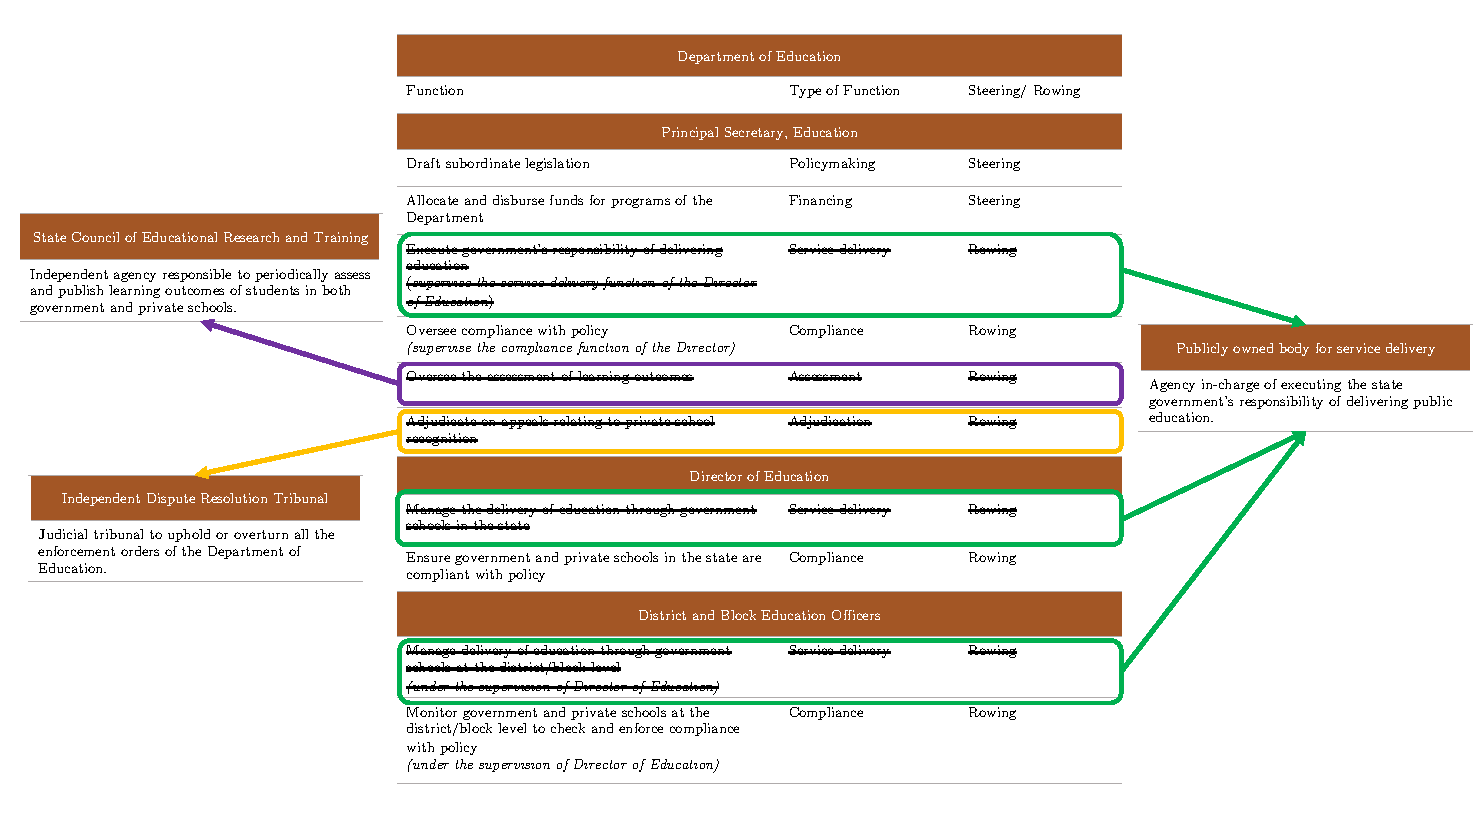
\includegraphics[page=1, width = 23.2cm]{figure5}
\caption{Education governance in India after \textit{uncoupling}}
\end{figure}
\end{landscape}

In 2018, both these schemes along with Scheme of Restructuring and Reorganisation of Teacher Education were subsumed under a composite scheme called Samagra Shiksha Abhiyan. This new composite scheme will be implemented through a newly formed State Implementation Society at the state level \parencite{smsa_pubjab}.\footnote{Names of the State Implementation Societies vary with different states.} 

We recommend that these newly formed State Implementation Societies, which are responsible for service delivery function, be completely independent from the state government’s Education Department. The department should not be involved in the service delivery functions of the new body but focus only on demanding accounting from this body and ensuring the compliance of schools and services managed by this independent body. 

The design features of the new body must include: 

\begin{enumerate}

\item \textbf{An independent governing board comprised of government and non-government members:} The new body should also be headed by a Governing Board, but its composition should have a combination of government and independent (non-government) members, with a predominance of independent members. Currently, the Board of Samagra Shiksha Abhiyan is dominated by government members.

\item \textbf{Clarity of responsibilities written into the institutional charter:} The agency should bear responsibility for all service delivery commitments of the state government under the RTE Act. The new agency should manage constructuring of government schools as per norms (both education and building construction regulations), maintain the correct pupil-teacher ratio in government schools, ensure admission of out-of-school children, provide remedial education, train teachers, appraise teacher performance, meet standards of learning outcomes, and deliver of mid-day meals, scholarships, free books, uniforms and regular health check-up of students in government schools.  
\end{enumerate}

%B. Establish a dispute resolution tribunal
\paragraph*{B. Establish a dispute resolution tribunal}
\addcontentsline{toc}{paragraph}{B. Establish a dispute resolution tribunal}

An independent tribunal to hear appeals against the rules drafted or the enforcement orders of a state government’s Education Department is essential to eliminate the violation of natural justice.

Today, orders of a state government’s Department of Education can be appealed through two channels: the department itself or through a court. Both these appeal channels have drawbacks: while adjudication by the department against its own orders is bad regulatory hygiene, approaching the Courts may result in inordinate delays. 

When TRAI was formed, it also adjudicated the appeals against itself. Therefore, the Telecom Dispute Settlement and Appellate Tribunal (TDSAT) was formed to address discomfort with such a design. The TDSAT now exclusively hears disputes between telecom companies, and between companies and TRAI.

Establishing an independent tribunal would also force the department to give more reasoned orders. Roy et al. \parencite*{roy_etal} writes about the transformation in the enforcement orders of Securities and Exchange Board of India (SEBI) after formation of Securities Appellate Tribunal (SAT).\footnote{When SEBI was first created in 1991, there was no possibility of appeal against a SEBI order in a neutral judicial forum. An appeal was to be made to the Government of India. In 1995, the SAT was created where some of SEBI orders (adjudication orders imposing monetary penalty) could be appealed \parencite{roy_etal}.} “In 1999, every order of SEBI became appealable in the SAT. It was a new experience for SEBI, to go from arbitrary power to the prospect of having numerous orders being scrutinised by SAT. However, over the years, this drove SEBI to higher levels of State capacity, towards higher quality work in the investigation, prosecution and quasi-judicial functions.”

%C. Repurpose SCERTs as independent assessment bodies
\paragraph*{C. Repurpose SCERTs as independent assessment bodies}
\addcontentsline{toc}{paragraph}{C. Repurpose SCERTs as independent assessment bodies}  

The SCERTs administer the National Achievement Survey to a student sample in every state to assess the learning outcomes \parencite{ncert_scert}. In addition, an SCERT conducts research to improve school education, designs curriculum, textbooks and courses and also assists the state government in academic matters.

Today, most SCERTs are under the administrative control of either the Principal Secretary of Education or Directorates of Education, who can exercise control over the assessments. Research shows that autonomy of the SCERT also has repercussions on their performance quality: “The need to ‘explain’ places restrictions on the SCERT/equivalent and this is passed downwards.”\footnote{GCERT is the equivalent of SCERT in the state of Gujarat, India.} The SCERTs that are more autonomous, like the Gujarat Council of Educational Research and Training (GCERT), produce superior research outputs and course materials. GCERT’s quality of teacher trainings, research, and relationship with the District Institute of Education and Training is attributed partly to the extent of its functional autonomy \parencite{scert_evidence}.

We argue that SCERTs should be released from the control of the state government Education Departments and repurposed to focus on student and teacher outcome assessments. The repurposed SCERTs could be designed using cues from the governance model of GCERT and the SCERT of Delhi, which are relatively autonomous agencies. These two SCERTs are constituted via a Memorandum of Association of the members who constitute their Governing Body and Executive Committee. The Governing Body lays down the direction of working and the Executive Committee implements the direction \parencite{del_scert}. The state Principal Secretary of Education chairs the Executive Committee and Director of the SCERT executes the daily activities \parencite{guj_scert_annualreport}. This last one however, we argue is a design flaw, and could impede governance unless high standards for accountability are written into the founding charter of the agency. 


%Who else has tried uncoupling in education?
\section*{Who else has tried \textit{uncoupling} in education?} 
\addcontentsline{toc}{section}{Who else has tried \textit{uncoupling} in education?} 

The application of separation of powers, and more specifically \textit{uncoupling}  is not alien to the governance systems of India. Service delivery and regulation in telecommunications and financial sectors, as also the production, transmission and distribution of electricity and water were uncoupled more than a decade ago. The application of separation of powers and \textit{uncoupling}has borne positive results for value for money of public spending as well as better outcomes for customers and consumers. 

In education, this principle has been thoroughly embedded in the systems of England and Chile and partially in Australia \parencite{aus_governance}, Denmark \parencite{denmarkgovernance}, Sweden\parencite{sweden_governance}, and Mexico \parencite{mex_governance}. 

%Example 1: Education Governance in the United Kingdom (UK)
\subsection*{Example 1: Education Governance in the United Kingdom (UK)}
\addcontentsline{toc}{subsection}{Example 1: Education Governance in the United Kingdom (UK)}

The State is the dominant provider of elementary education in the UK; students who attend fee-paying ‘independent schools’ or homeschool account for only seven percent of the school-age population. The Department for Education (DfE) is central authority that oversees education in the country, and is supported by 18 independent agencies \parencite{dfe}. 

The DfE’s primary responsibility is policy-formulation and allocation of responsibilities to the 18 distinct agencies.\footnote{Other non-prominent steering functions of regulating teaching profession, minimum learning levels etc. are performed by the other regulation agencies, as they require subject expertise.} Service delivery is done through public schools financed by Local Education Authorities. Compliance is ensured by two inspecting agencies—Office of Qualifications and Examinations Regulation (OFQUAL) and Office for Standards in Education (OFSTED)—which report directly to the Parliament. Certain aspects of compliance are further subdivided to create more focused agencies and streamline governance. Table 1 provides an overview of the governance of education in the UK.


{\small
\begin{longtable}{>{\raggedright}p{3.5cm}>{\raggedright}p{7.8cm}>{\raggedright\arraybackslash}p{3cm}}
\caption{Functions of the Department for Education in the UK and some of the agencies housed under it
} \\
\toprule
\multicolumn{3}{c}{Department for Education (Steering)} \\
\midrule
\multicolumn{3}{l}{\tabitem Formulate education policy for the country}  \\
\multicolumn{3}{l}{\tabitem Allocate responsibilities to each of the 18 agencies and oversee their performance}  \\

\midrule
\endfirsthead
 Agency & Function \\ {\footnotesize\textit{(description of each agency from its website)}} & Type of Function  \\
\toprule
\endhead
\endlastfoot
Agency & Function  \\ {\footnotesize\textit{(description of each agency from its website)}} & Type of Function \\
\midrule
OFQUAL & Regulates qualifications, examinations and assessments & Rowing (compliance) \\
 & & \\
OFSTED & Inspects and regulates services that provide education and skills to learners of all ages & Rowing (compliance) \\
 & & \\
Education and Skills Funding Agency & Distributes funding for education and skills for children, young people and adults & Rowing \newline (service delivery) \\
  & & \\
Standards and Testing Agency & Sets tests to assess children in the education system & Rowing \newline (assessment) \\
 & & \\
Higher Education Funding Council for England & Distribution of funding to universities and colleges for teaching and research & Rowing \newline (service delivery) \\
 & & \\
Office for Fair Access & Safeguards and promotes fair access to higher education by approval and monitoring of universities that want to charge higher fees & Rowing (compliance) \\
 & & \\
Student Loans Company & Administers loans and grants to university students and colleges in the UK & Rowing \newline (service delivery) \\
 & & \\
School Teachers’ Review Body & Recommends pay, duties, and working time of the school teachers & Steering\footnotemark \\
\bottomrule

\end{longtable}}
\footnotetext{The steering function is ‘advisory to the DfE’ and is non-binding.}

%Example 2: Education Governance in Chile
\subsection*{Example 2: Education Governance in Chile}
\addcontentsline{toc}{subsection}{Example 2: Education Governance in Chile} 

The Ministry of Education (MoE) is the central authority that oversees education in the country; governance is also shared with the local authorities. In 2012 Chile passed a new law called National System for the Assurance of the Quality of Parvular (Kindergarten), Basic and Medium Education and its Supervision. The law applied separation of powers and \textit{uncoupling}, and reassigned many of MoE’s functions to other agencies. It also created two new agencies for better enforcement and accountability—Superintendence of Education, and the Education Quality Assurance Agency (\cite{nhlpc_chile}; \cite{chile_ed_policy}).

Municipality-operated and privately-owned schools are the service deliverers, who are financed through a per-student funding model of vouchers. Schools are expected to comply with regulations, be accountable to the resources received, allow assessment of education quality and request and receive support for quality improvement.

\newpage
%Table
{\small
\begin{longtable}{>{\raggedright}p{7.5cm}>{\raggedright\arraybackslash}p{7.7cm}}
\caption{A pre and post reform comparison of Chile’s Education governance} \\
\toprule
Before & After \\
\midrule
\endfirsthead
Before & After \\
\midrule
\endhead
\multicolumn{2}{r}{{Continued\ldots}} \
\endfoot
\hline
\endlastfoot

\multicolumn{2}{c}{(Ministry of Education  (Steering)} \\
\midrule
\tabitem Propose and implement education policy \newline 
\tabitem Enforce educational rules and regulations \newline
\tabitem Address complaints \newline
\tabitem Develop curriculum, study plans and study programs \newline
\tabitem Organise evaluations and international studies \newline
\tabitem Register relevant information. & \tabitem Govern the new system and the agencies \newline
\tabitem Propose and implement education policy. \\
\midrule
\multicolumn{2}{c}{National Council of Education (Steering)} \\
\midrule
\tabitem Approve curriculum, study plans and study programs. & \tabitem Design, develop and approve curriculum, study plans and study programs; \newline \tabitem Set learning standards, performance standards of principals and teachers, quality indicators in the system and assessment plan. \\
\midrule
\multicolumn{2}{c}{Superintendence of Education (Compliance)} \\
\midrule
\multicolumn{2}{l}{\tabitem Enforce educational laws, rules and regulations} \\
\multicolumn{2}{l}{\tabitem Supervise the legality in the use of public resource} \\ 
\multicolumn{2}{l}{\tabitem Audit the accountability in the system } \\
\multicolumn{2}{l}{\tabitem Adjudicate complaints and disputes.}  \\
\midrule
\multicolumn{2}{c}{Education Quality Assurance Agency (Assessment)} \\
\midrule
\multicolumn{2}{l}{\tabitem Assess learning achievements of students, and other quality indicators of the school} \\
\multicolumn{2}{l}{\tabitem Classify schools according to learning achievements and other quality indicators} \\
\multicolumn{2}{l}{\tabitem  Provide guidelines for improvement of the education quality in the schools.} 

\end{longtable}}


\newpage
%Conculsion
\section*{Conclusion}
\addcontentsline{toc}{section}{Conclusion} 

State government Education Departments in India perform at least six incompatible functions. This overlap of functions and responsibilities has resulted in several systemic challenges and compromised our education quality. The solution to these problems lies not in marginal improvements, but in significant restructuring of the governance system. 

Government schools in India lack any independent oversight and are self-regulated by the department. This flawed accountability structure promotes conflicts of interest. This Blueprint proposes that government schools be managed by an independent publicly owned organisation, and a state government Education Department concern itself with the strict enforcement of laws and standards in the case of both government or private schools. Similarly the functions of adjudication and assessment ought to be managed by agencies independent from the department.

Such measures were taken some decades ago in the telecommunications and securities sector. As a result, the benefits of due process, fast innovation, widespread access and low consumer costs have accrued down to the poorest. It is imperative that we similarly reform the education sector to innovate and improve. 

India performed abysmally on PISA in 2009. Ever since, learning outcomes for all children have only fallen. India has committed to participate in PISA 2021, but only an overhaul of the governance of education will save us from repeat embarrassment. 

Separation of Powers is the cornerstone of these reforms. This Blueprint outlines an \textit{uncoupling} approach to implementing separation of powers, functions and roles in education governance. The framework it provides is only a starting step to think practically about restructuring our education system. Redesigning state government Education Departments to focus on rule making and enforcement, and setting up independent agencies to hold responsibility for assessment, adjudication and service delivery, requires careful thought. Each design choice will have implications downstream. The key questions that should guide the restructuring though remain: whether the system upholds rule of law, provides value for money for public spending, and achieves outcome goals. 
\newpage
%Bibliography
\section*{Bibliography}
\addcontentsline{toc}{section}{Bibliography}
\printbibliography[heading=none] 

\newpage
\pagenumbering{gobble} %removes page numbers starting here
\pagestyle{empty} %removes footers from here onwards
\includepdf[pages={5,6}, pagecommand={}]{Coverpage.pdf}

                                        
\end{document}